\documentclass{beamer}

%\usepackage{movie15}
\usepackage{verbatim}
\usepackage{amsmath}

\usepackage{tikz}
\usetikzlibrary{shapes, arrows, calc}

\usepackage[T1]{fontenc}
\usepackage[ansinew]{inputenc}
\usepackage{lmodern} 
\usepackage{textcomp}

\useoutertheme{infolines} 
\setbeamertemplate{navigation symbols}{}
\setbeamertemplate{items}[ball] 
\setbeamertemplate{blocks}[rounded][shadow=true] 

%\usetheme{Boadilla}
\usetheme{Madrid}
\usecolortheme{whale}

\author[Boshen Chen]{Boshen Chen \\{\small Supervised by: Dr.\ Andrea Raith, Olga Perederieieva}}

\title[Faster Shortest Path Computation]{Faster Shortest Path Computation for Traffic Assignment}

%\subtitle[]{}

\institute[UoA]{
    Department of Engineering Science\\
    University of Auckland\\
}

\date{}

\begin{document}

\begin{frame}[plain]
    \titlepage
\end{frame}

%\begin{frame}{Contents}
%    \tableofcontents
%\end{frame}

\section{Project motivation - Traffic Assignment}
\begin{frame}{Traffic Assignment}
    \pause
    \begin{itemize}[<+->]
        \item transportation network with supply and demand nodes
        \item minimise travel times
        \item arcs have non-linear travel times for capturing congestion effects
        %\item all-or-nothing assignment
        %    \begin{itemize}
        %        \item send traffic all at once to a node via the shortest path
        %    \end{itemize}
    \end{itemize}

    %\pause
    \uncover<4->{
        \begin{center}
            \tikzstyle{block} = [rectangle, draw, text width=.5\paperwidth, text centered, rounded corners, minimum height=2em]
            \tikzstyle{line} = [draw, -latex']
            \begin{tikzpicture}[node distance=4em]
                \uncover<5->{
                    \node [block] (first) {Initialise: load all traffic on shortest path with free flow travel times};
                }

                \uncover<6->{
                    \node [block, below of=first] (second) {Update travel times};
                    \path [line] (first) -- (second);
                }

                \uncover<7->{
                    \node [block, below of=second] (third) {Reload traffic on shortest path with new travel times};
                    \path [line] (second) -- (third);
                }

                \uncover<8->{
                    \node [block, below of=third] (fourth) {Check stopping criterion (equilibrium)};
                    \path [line] (third) -- (fourth);
                }
                % none of the travellers can find a faster rote than the one he is currently using

                \uncover<9->{
                    \path [line] (fourth.west) -- ($(fourth.west)-(0.8,0)$) -- ($(second.west)-(0.8,0)$) -- (second.west);
                }
            \end{tikzpicture}
        }
    \end{center}

\end{frame}
\begin{comment}
\begin{frame}{Transportation forecasting}

    \begin{columns}
        \begin{column}{0.5\paperwidth}
            \begin{center}
                \tikzstyle{block} = [rectangle, draw, text width=10em, text centered, rounded corners, minimum height=2em]
                \tikzstyle{line} = [draw, -latex']
                \begin{tikzpicture}[node distance=4em]
                    \pause

                    \node [block] (first) {Trip Generation};
                    \pause

                    \node [block, below of=first] (second) {Trip Distribution};
                    \path [line] (first) -- (second);
                    \pause

                    \node [block, below of=second] (third) {Mode Choice};
                    \path [line] (second) -- (third);
                    \pause

                    \node [block, below of=third] (fourth) {Traffic Assignment};
                    \path [line] (third) -- (fourth);
                    \pause

                    \path [line] (fourth.west) -- ($(fourth.west)-(0.8,0)$) -- ($(first.west)-(0.8,0)$) -- (first.west);
                    \path [line] ($(second.west)-(0.8,0)$) -- (second.west);
                    \path [line] ($(third.west)-(0.8,0)$) -- (third.west);
                \end{tikzpicture}
            \end{center}
        \end{column}

        %\begin{column}{0.5\paperwidth}
        %    What has been done in the past \ldots
    % mo%tivation, transportation forecasting and the 4 stage modelling process
    % us%e figure
        %    \begin{itemize}
        %        \item trip generation
        %        \item trip distribution
        %        \item mode choice
        %        \item traffic assignment
        %    \end{itemize}

        %    Traffic assignment
        %    \begin{itemize}
        %        \item how its solved
        %        \item concept of user equilibrium
        %        \item shortest path calculations
        %        \item link cost, lots of iterations, each iteration lots of shortest path calculations
        %    \end{itemize}
        %\end{column}
    \end{columns}

\end{frame}
\end{comment}

\section{Solving the Traffic Assignment problem - faster shortest path calculations}
\begin{frame}[shrink]{The Graph - 93,135 Origin-Destination Pairs}
    % Let me go through the steps I took to find a faster algorithm,
    % on this graph with more than 93,000 origin destination pairs
    \begin{center}
        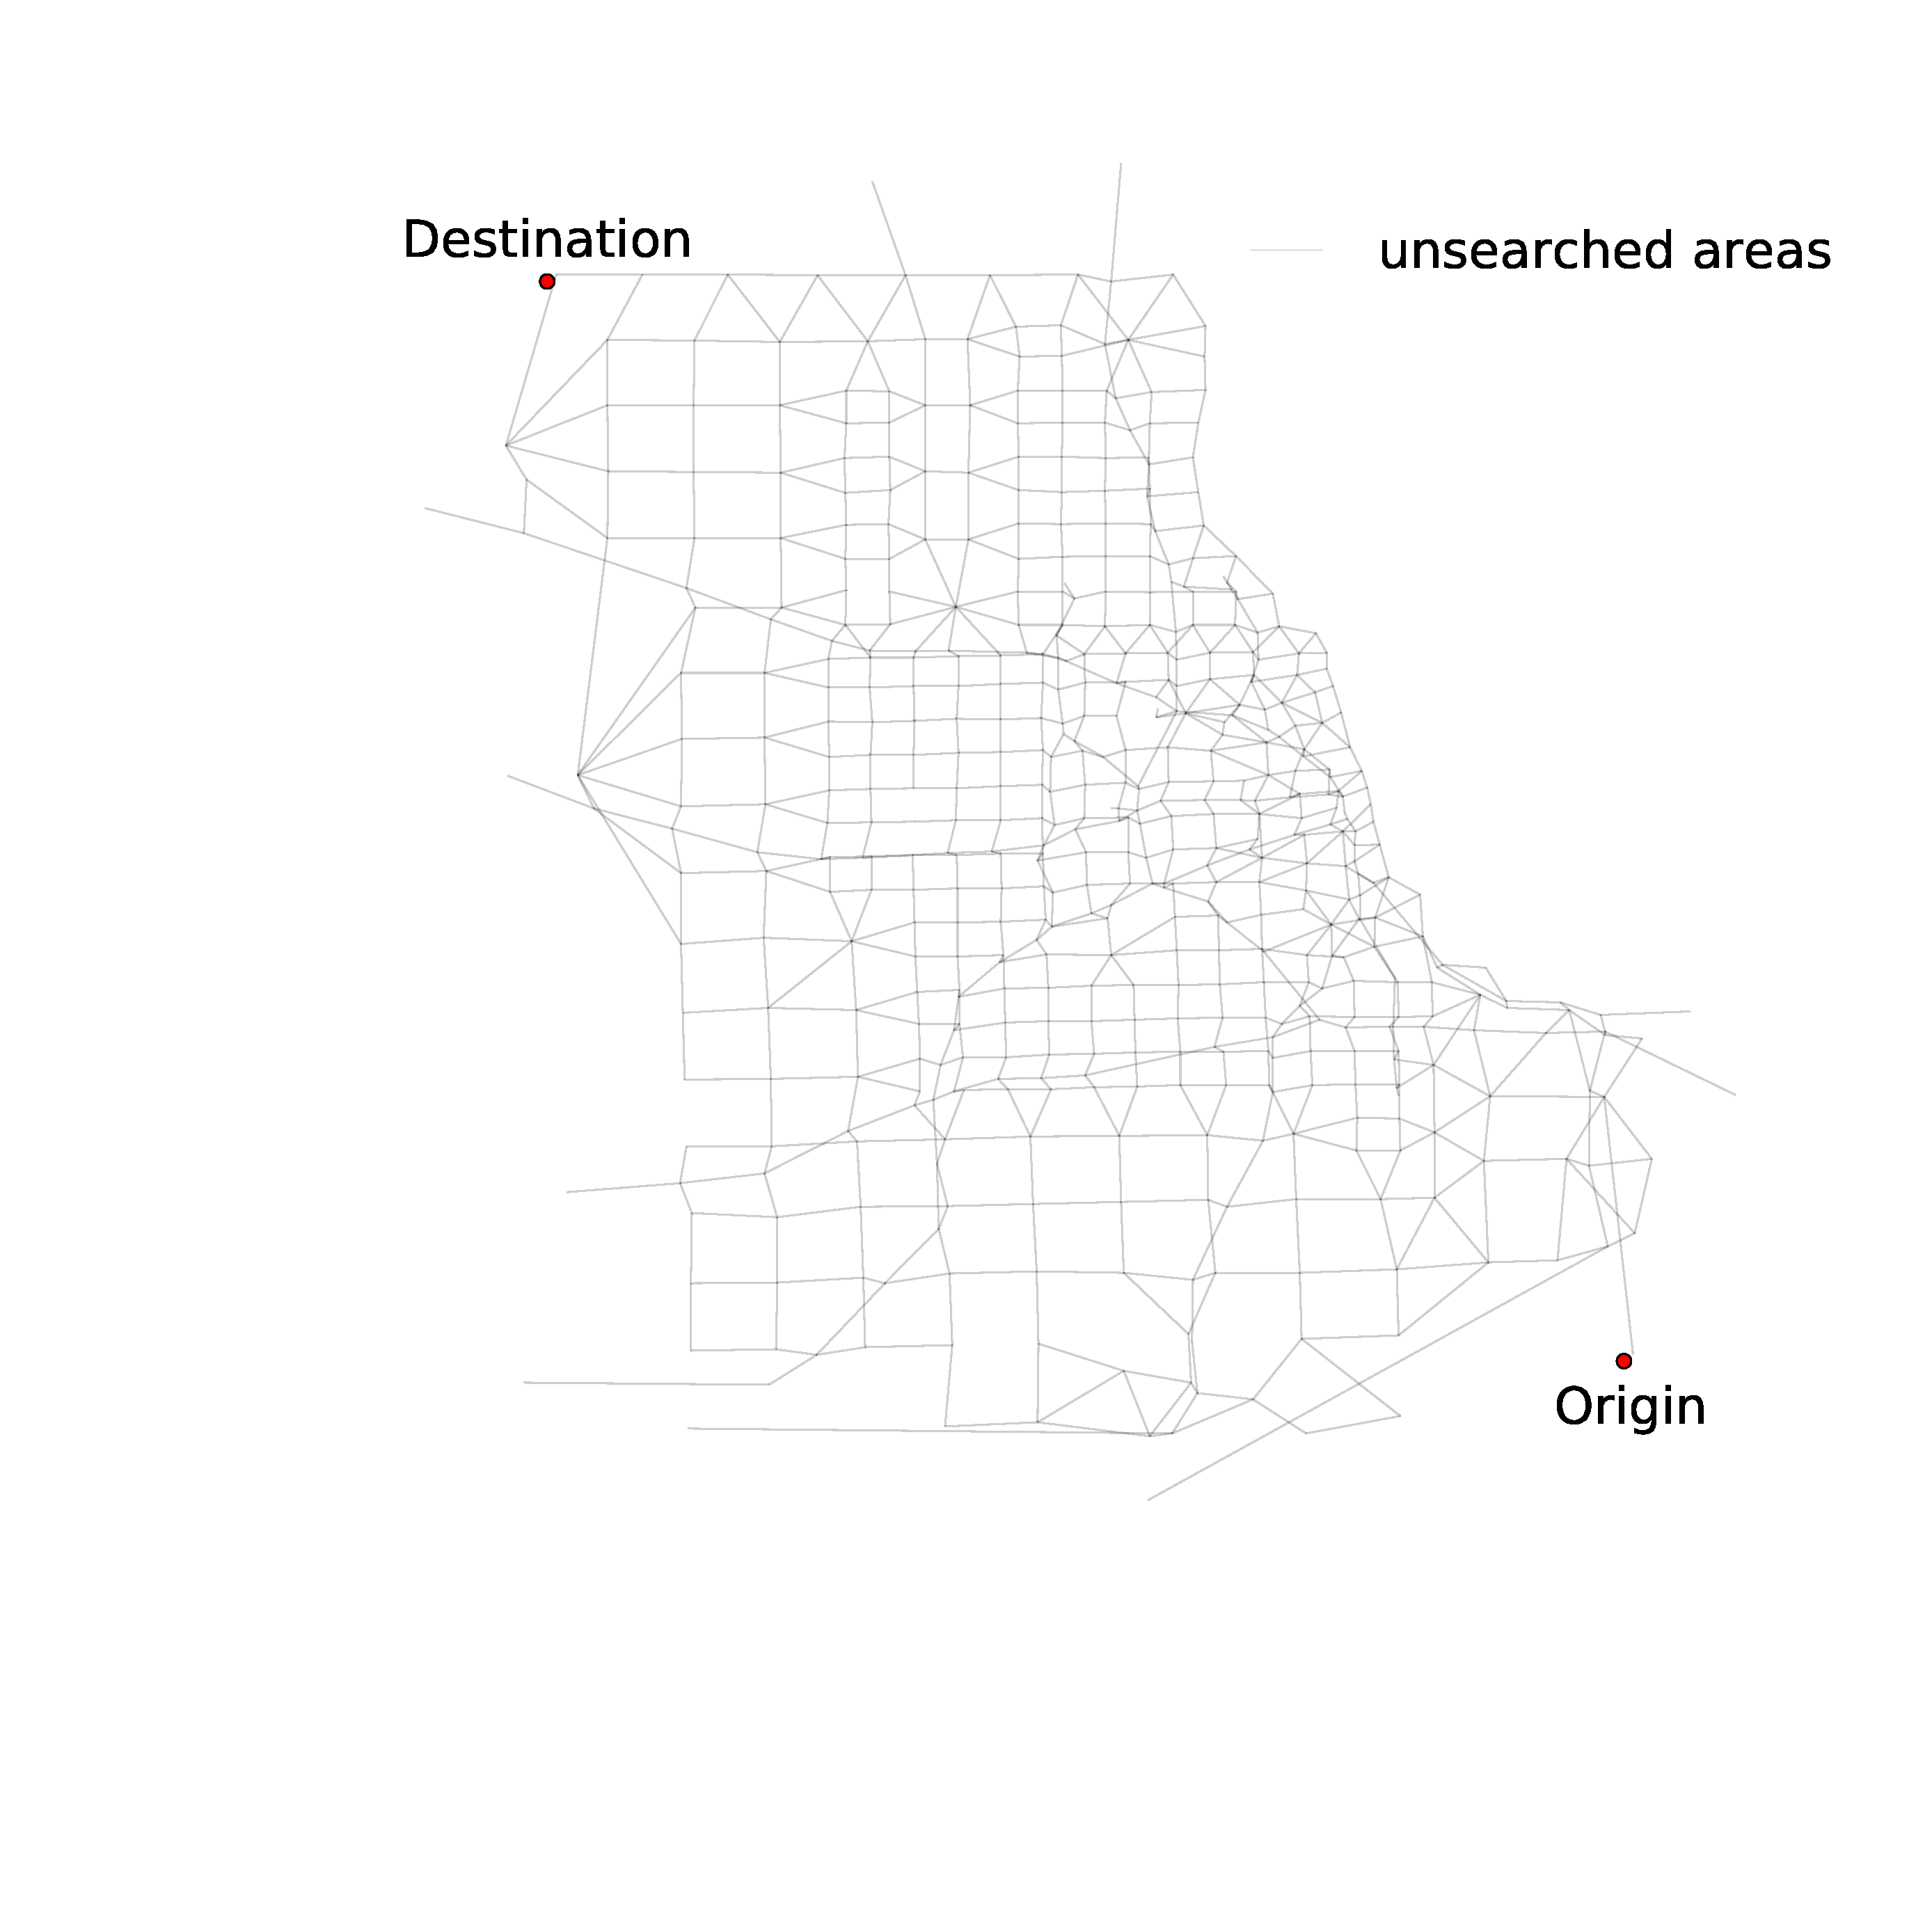
\includegraphics[page=1,width=\paperwidth, height=\paperheight, keepaspectratio,trim=0 120px 48px 120px,clip]{img/chicago_dijkstra_animation}
    \end{center}
\end{frame}

\begin{comment}
\begin{frame}{Faster shortest path calculations}

    What exist and what I have done \ldots
    \begin{itemize}
        \item Bellman Ford - label correcting algorithm
        \item Dijkstra - label setting algorithm
            \begin{itemize}
                \item different data structures - Heap trees and their advantages
            \end{itemize}
        \item bidirectional
        \item A* search
        \item bidirectional A* search
        \item preprocessing
    \end{itemize}

\end{frame}
\end{comment}

\begin{frame}[shrink]{Dijkstra's Algorithm}
    \foreach \n in {1,...,7}{
        \only<\n>{
            \begin{center}
                \includegraphics[page=\n,width=\paperwidth, height=\paperheight, keepaspectratio,trim=0 120px 48px 120px,clip]{img/chicago_dijkstra_animation}
            \end{center}
        }
    }
\end{frame}

% can talk about data structure here
\begin{frame}{Dijkstra's Algorithm - Priority Queue}
    \begin{itemize}
        \item pointer based Heap (C++ boost library)
            \begin{itemize}
                \item Binomial
                \item Pairing
                \item Binary
                \item Ternary
                \item Skew
                \item Fibonacci
            \end{itemize}
        \item (red-black) binary search tree (C++ STL <set>)
        \item array based Heap (C++ STL <priority\_queue>)
    \end{itemize}
\end{frame}

\begin{frame}[shrink]{Dijkstra's Algorithm - Priority Queue}
    \begin{center}
        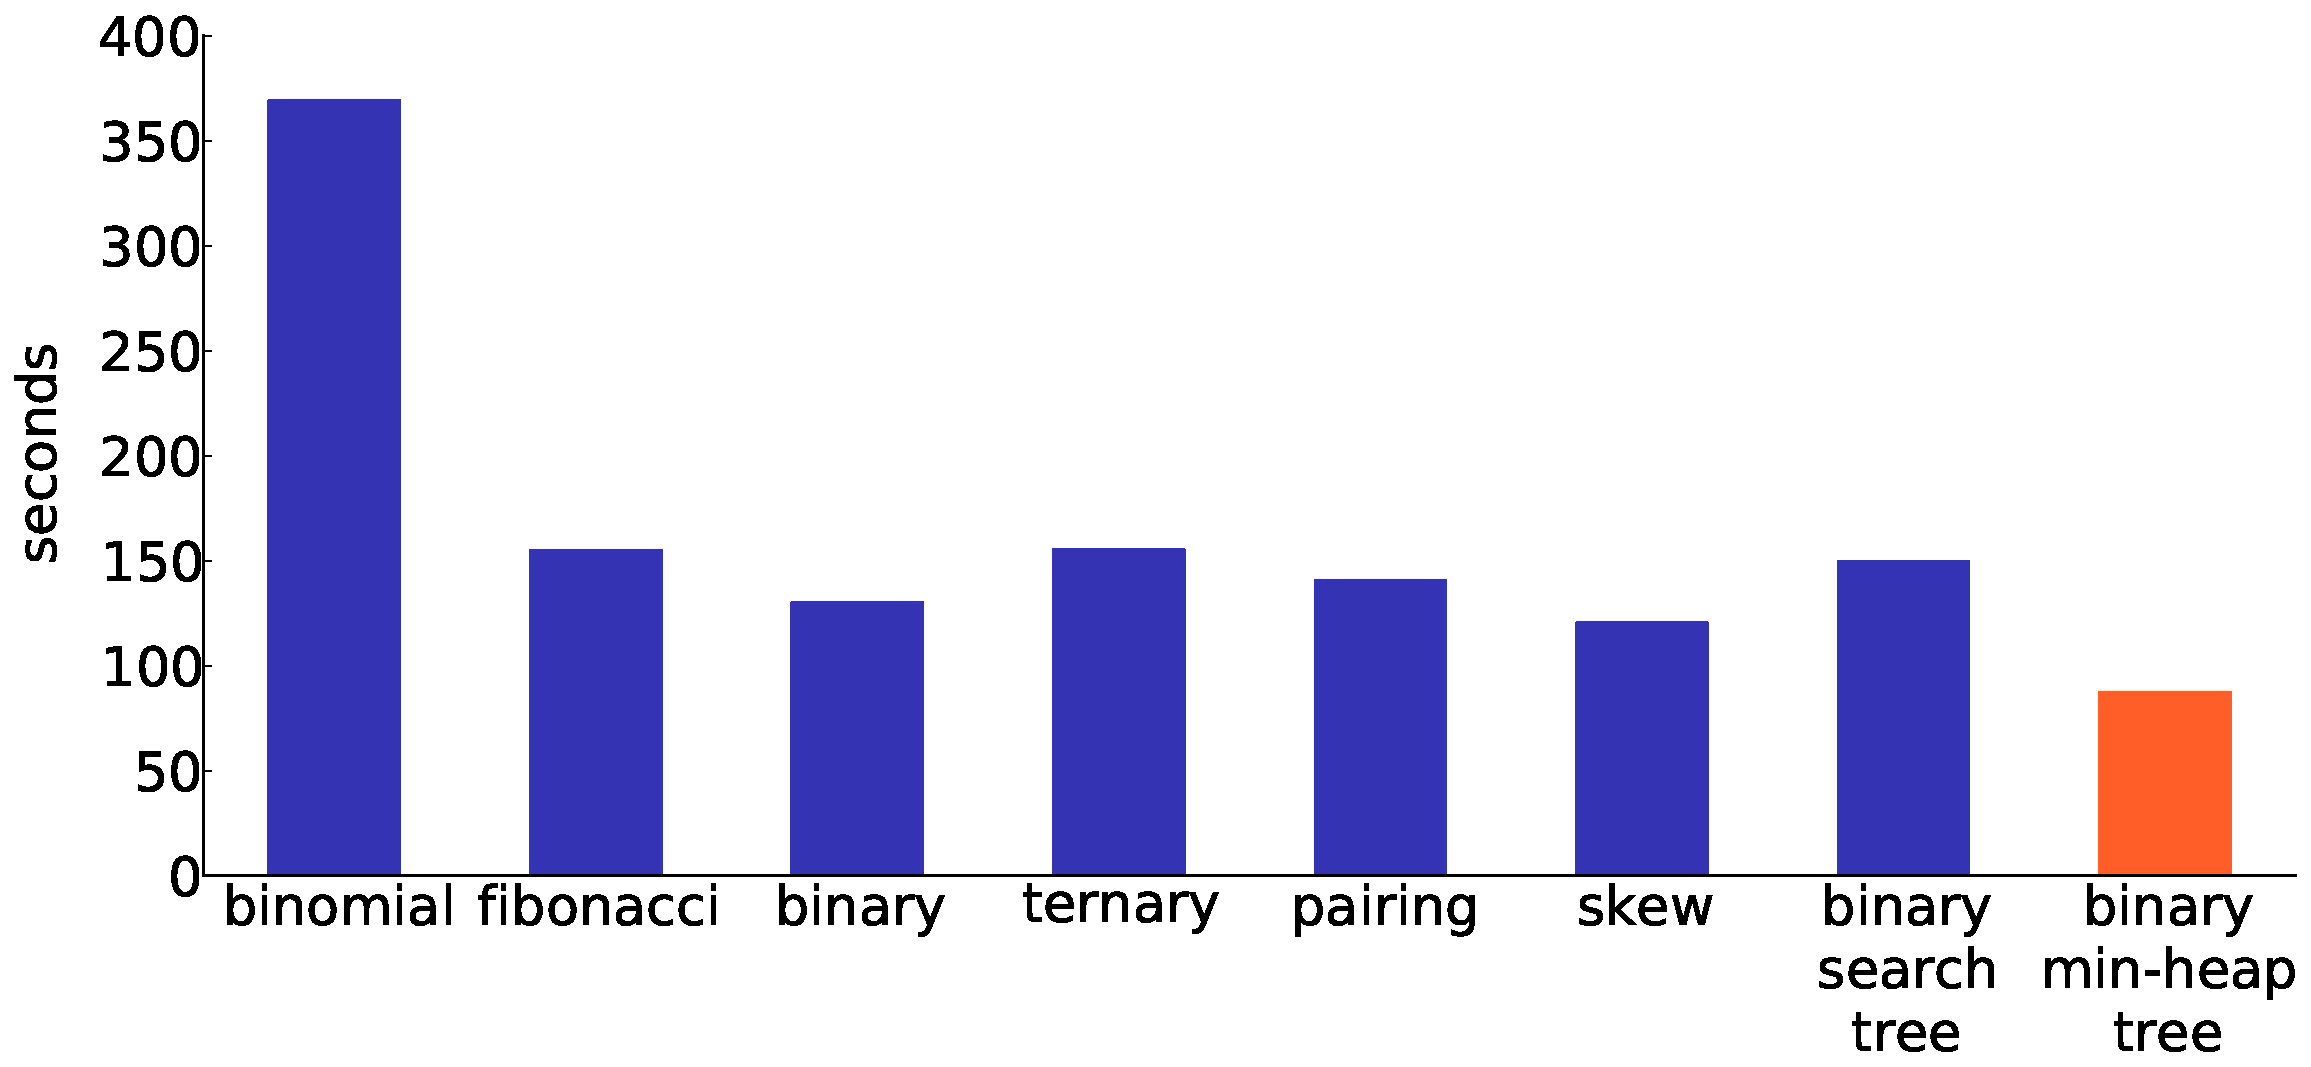
\includegraphics[width=\paperwidth, height=\paperwidth, keepaspectratio, trim=0 0 0 25pt, clip]{img/pq_runtime}
    \end{center}
\end{frame}

% since we have a origin and a destination, 
% we can calculate from the two ends 
\begin{frame}[shrink]{Bidirectional Dijkstra's Algorithm}
    \foreach \n in {1,...,7}{
        \only<\n>{
            \begin{center}
                \includegraphics[page=\n,width=\paperwidth, height=\paperheight, keepaspectratio,trim=0 120px 48px 120px,clip]{img/chicago_bidirect_animation}
            \end{center}
        }
    }
\end{frame}

\begin{frame}[shrink]{A* Search (Best-First Search)}
    \begin{itemize}
        \item Visit the next node that is on the expected shortest path.
    \end{itemize}
    \foreach \n in {1,...,5}{
        \only<\n>{
            \begin{center}
                \includegraphics[page=\n,width=\paperwidth, height=\paperheight, keepaspectratio,trim=0 120px 48px 120px,clip]{img/chicago_astar_animation}
            \end{center}
        }
    }
\end{frame}

\begin{frame}[shrink]{Bidirectional A* search}
    \foreach \n in {1,...,7}{
        \only<\n>{
            \begin{center}
                \includegraphics[page=\n,width=\paperwidth, height=\paperheight, keepaspectratio,trim=0 120px 48px 120px,clip]{img/chicago_astar_bidirect_animation}
            \end{center}
        }
    }
\end{frame}

\section{Results - speed ups}
\begin{frame}
    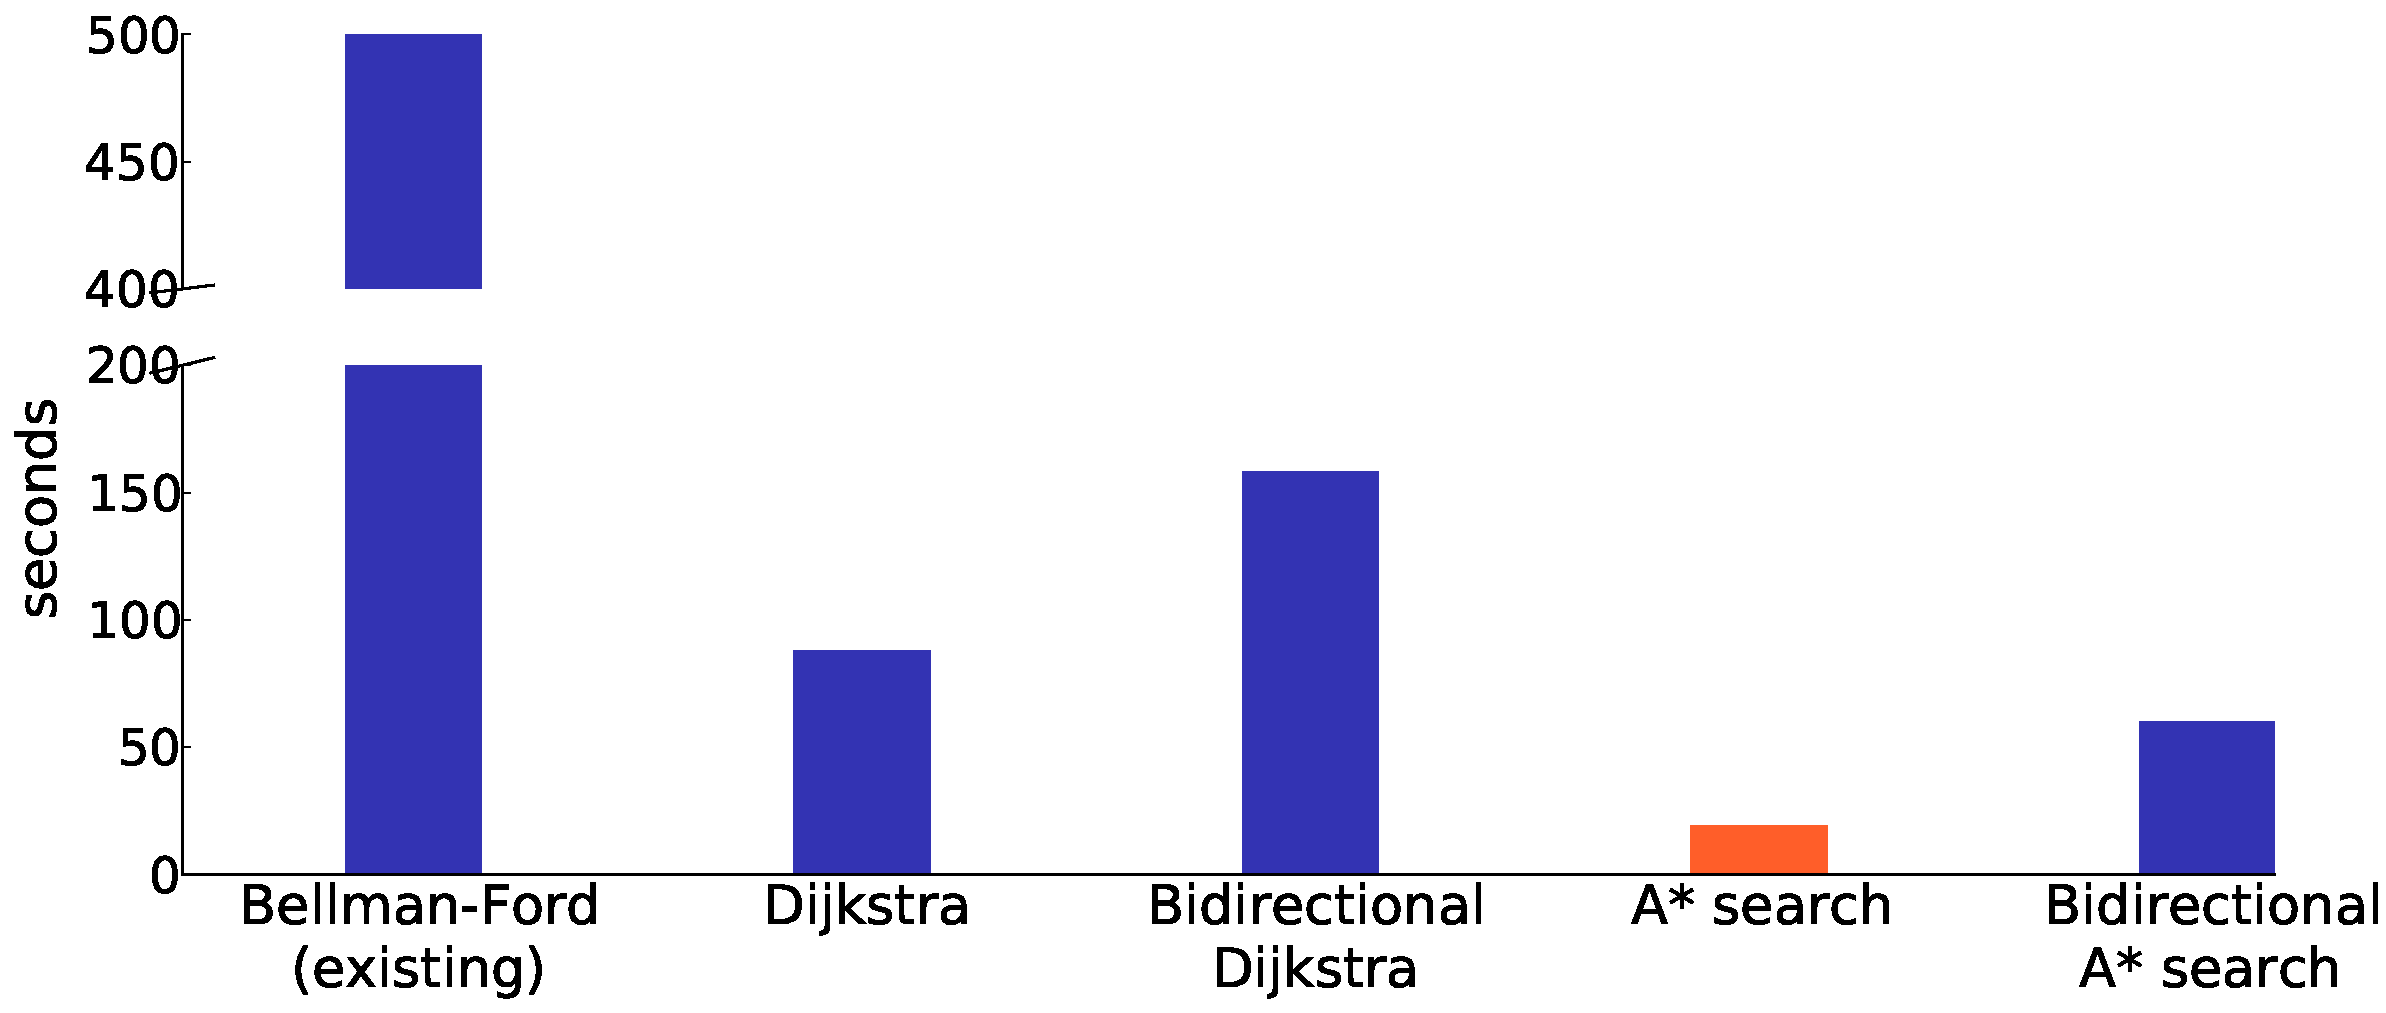
\includegraphics[width=\paperwidth, height=\paperheight, keepaspectratio, trim=0 0 0 60pt, clip]{img/runtime}
    \tikzstyle{block} = [circle, draw, inner sep=0pt,minimum size=1pt]
    \begin{tikzpicture}[overlay, shift={(1.6,0)}]
        \node [block, minimum size= 1.4pt] (a) {};
        \node [block, minimum size= 7.9pt] (b) [xshift=-0.1cm, right of=a] {};
        \node [block, minimum size= 4.3pt] (c) [xshift=0.4cm, right of=b] {};
        \node [block, minimum size= 93pt] (d) [xshift=6.7cm, right of=c] {};

        \node [above] at (a.north) {\tiny 10 iters};
        \node [above] at (b.north) {\tiny 27 iters};
        \node [above] at (c.north) {\tiny 126 iters};
        \node [above] at (d) {\tiny 25 iters};
    \end{tikzpicture}
\end{frame}

\begin{frame}{Future Work}
    \begin{itemize}[<+->]
        \item preprocessing
            \begin{itemize}
                \item A* search combined with landmark distances
            \end{itemize}
        \item use information from previous iteration
            \begin{itemize}
                \item Incremental heuristic search - Lifelong Planning A*
            \end{itemize}
        \item avoid shortest path calculations if possible
            \begin{itemize}
                \item most of the shortest paths do not change after the first few iterations
            \end{itemize}
        % fix shortest path tree if altered somewhere
    \end{itemize}
\end{frame}
\end{document}
